\PassOptionsToPackage{table}{xcolor}
\documentclass[aspectratio=169]{beamer}\usepackage[utf8]{inputenc}
\usepackage{lmodern}
\usepackage[english]{babel}
\usepackage{color}
\usepackage{amsmath,mathtools}
\usepackage{booktabs}
\usepackage{mathptmx}
\usepackage[11pt]{moresize}
\usepackage{hyperref}
\usepackage{commath}
\usepackage{bm}
\usepackage{subfigure}
\usepackage{siunitx}

\setbeamertemplate{navigation symbols}{}
\setbeamersize{text margin left=5mm,text margin right=5mm}
\setbeamertemplate{caption}[numbered]
\addtobeamertemplate{navigation symbols}{}{
\usebeamerfont{footline}
\usebeamercolor[fg]{footline}
\hspace{1em}
\insertframenumber/\inserttotalframenumber}

\newcommand{\R}{\mathbb{R}}
\newcommand{\E}{\mathbb{E}}
\newcommand{\N}{\mathbb{N}}
\newcommand{\Z}{\mathbb{Z}}
\newcommand{\V}{\mathbb{V}}
\newcommand{\Q}{\mathbb{Q}}
\newcommand{\K}{\mathbb{K}}
\newcommand{\C}{\mathbb{C}}
\newcommand{\T}{\mathbb{T}}
\newcommand{\I}{\mathbb{I}}

\title{Small Report}
\subtitle{Renzo Miguel Caballero Rosas}

\begin{document}

\begin{frame}
\titlepage
\end{frame}

%%%%%%%%%%%%%%%%%%%%%%%%%%%%%%%%%%%

\setbeamercolor{background canvas}{bg=white!10}
\begin{frame}\frametitle{Iterations triangle-triangle}

\begin{columns}[c]

\column{.4\textwidth}
Let $C_0$ the first triangular pulley and $C_{n+1}=f(C_n)$ the process of printing the next triangular designed pulley $C_{n+1}$ using the printed triangular designed pulley $C_n$.\\
\quad\\
In the picture we can see $C_i$ with $i\in\{1,\dots,6\}$.

\column{.6\textwidth}
\begin{figure}[ht!]
\centering
\includegraphics[width=1\textwidth]{20201221_152845.jpg}
\end{figure}

\end{columns}

\end{frame}

%%%%%%%%%%%%%%%%%%%%%%%%%%%%%%%%%%%

\setbeamercolor{background canvas}{bg=white!10}
\begin{frame}\frametitle{Iterations triangle-triangle}

\begin{columns}[c]

\column{.4\textwidth}
In the picture, we can notice the deformation in the cylindrical bases of
\begin{table}[]
\begin{tabular}{lll}
$C_1$ & $C_2$ & $C_3$ \\
$C_4$ & $C_5$ & $C_6$.
\end{tabular}
\end{table}
It may be necessary more iterations to find a pattern. But we can observe an improvement in the shape from $C_4$ to $C_5$.

\column{.6\textwidth}
\begin{figure}[ht!]
\centering
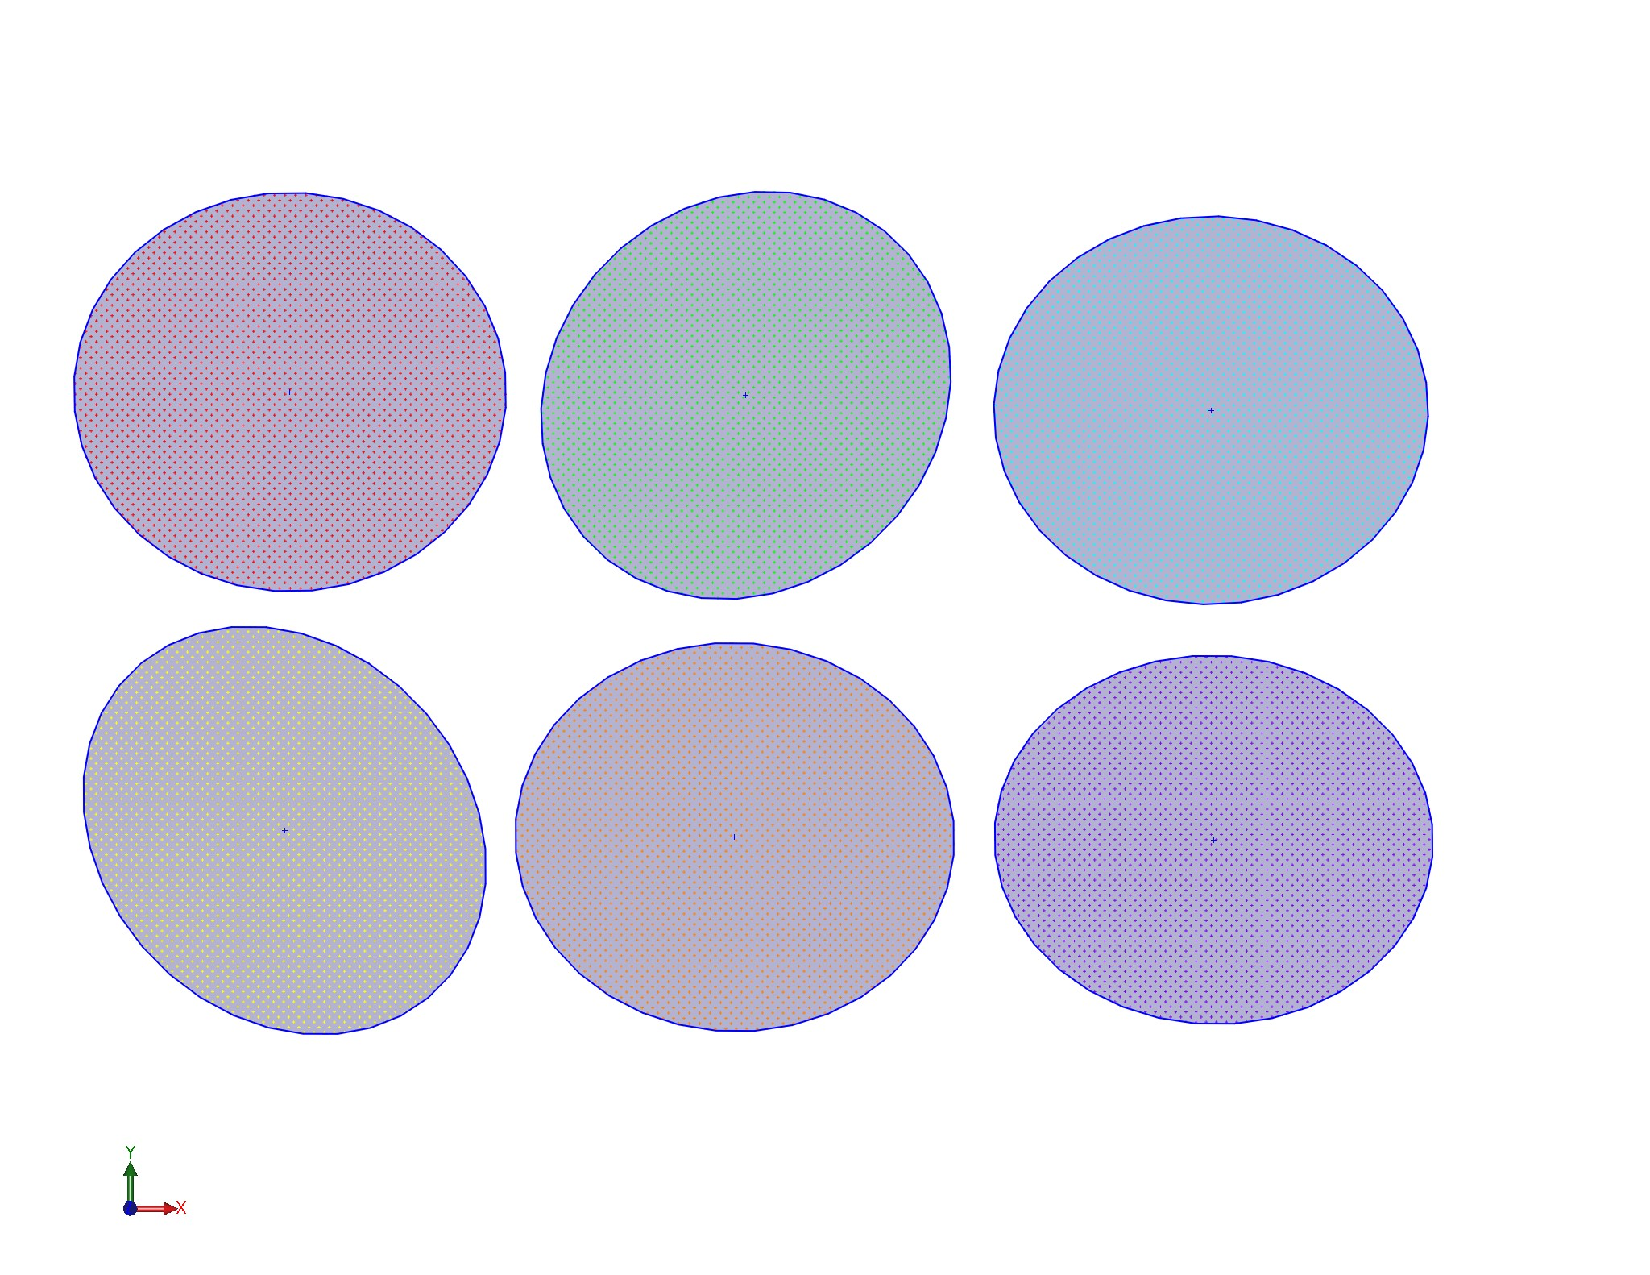
\includegraphics[width=1\textwidth]{circles_2.jpg}
\end{figure}

\end{columns}

\end{frame}

%%%%%%%%%%%%%%%%%%%%%%%%%%%%%%%%%%%

\setbeamercolor{background canvas}{bg=white!10}
\begin{frame}\frametitle{Iterations triangle-triangle}

\begin{columns}[c]

\column{.5\textwidth}
In the picture, we can see the triangular shape of {\color{red}$C_0$} and {\color{blue}$C_7$}.

\column{.5\textwidth}
\begin{figure}[ht!]
\centering
\includegraphics[width=0.9\textwidth]{triangle.jpg}
\end{figure}

\end{columns}

\end{frame}

%%%%%%%%%%%%%%%%%%%%%%%%%%%%%%%%%%%

\setbeamercolor{background canvas}{bg=white!10}
\begin{frame}\frametitle{Possible future step}

\begin{columns}[c]

\column{.5\textwidth}
We can identify the step motors' controllers (A4988) in the printer's motherboard. If we can substitute the main controller, ATMEGA1284P, we can modify the printer's software. It can be reasonable to spend some time on this and see if it can be done.\\
\quad\\
\begin{figure}[ht!]
\centering
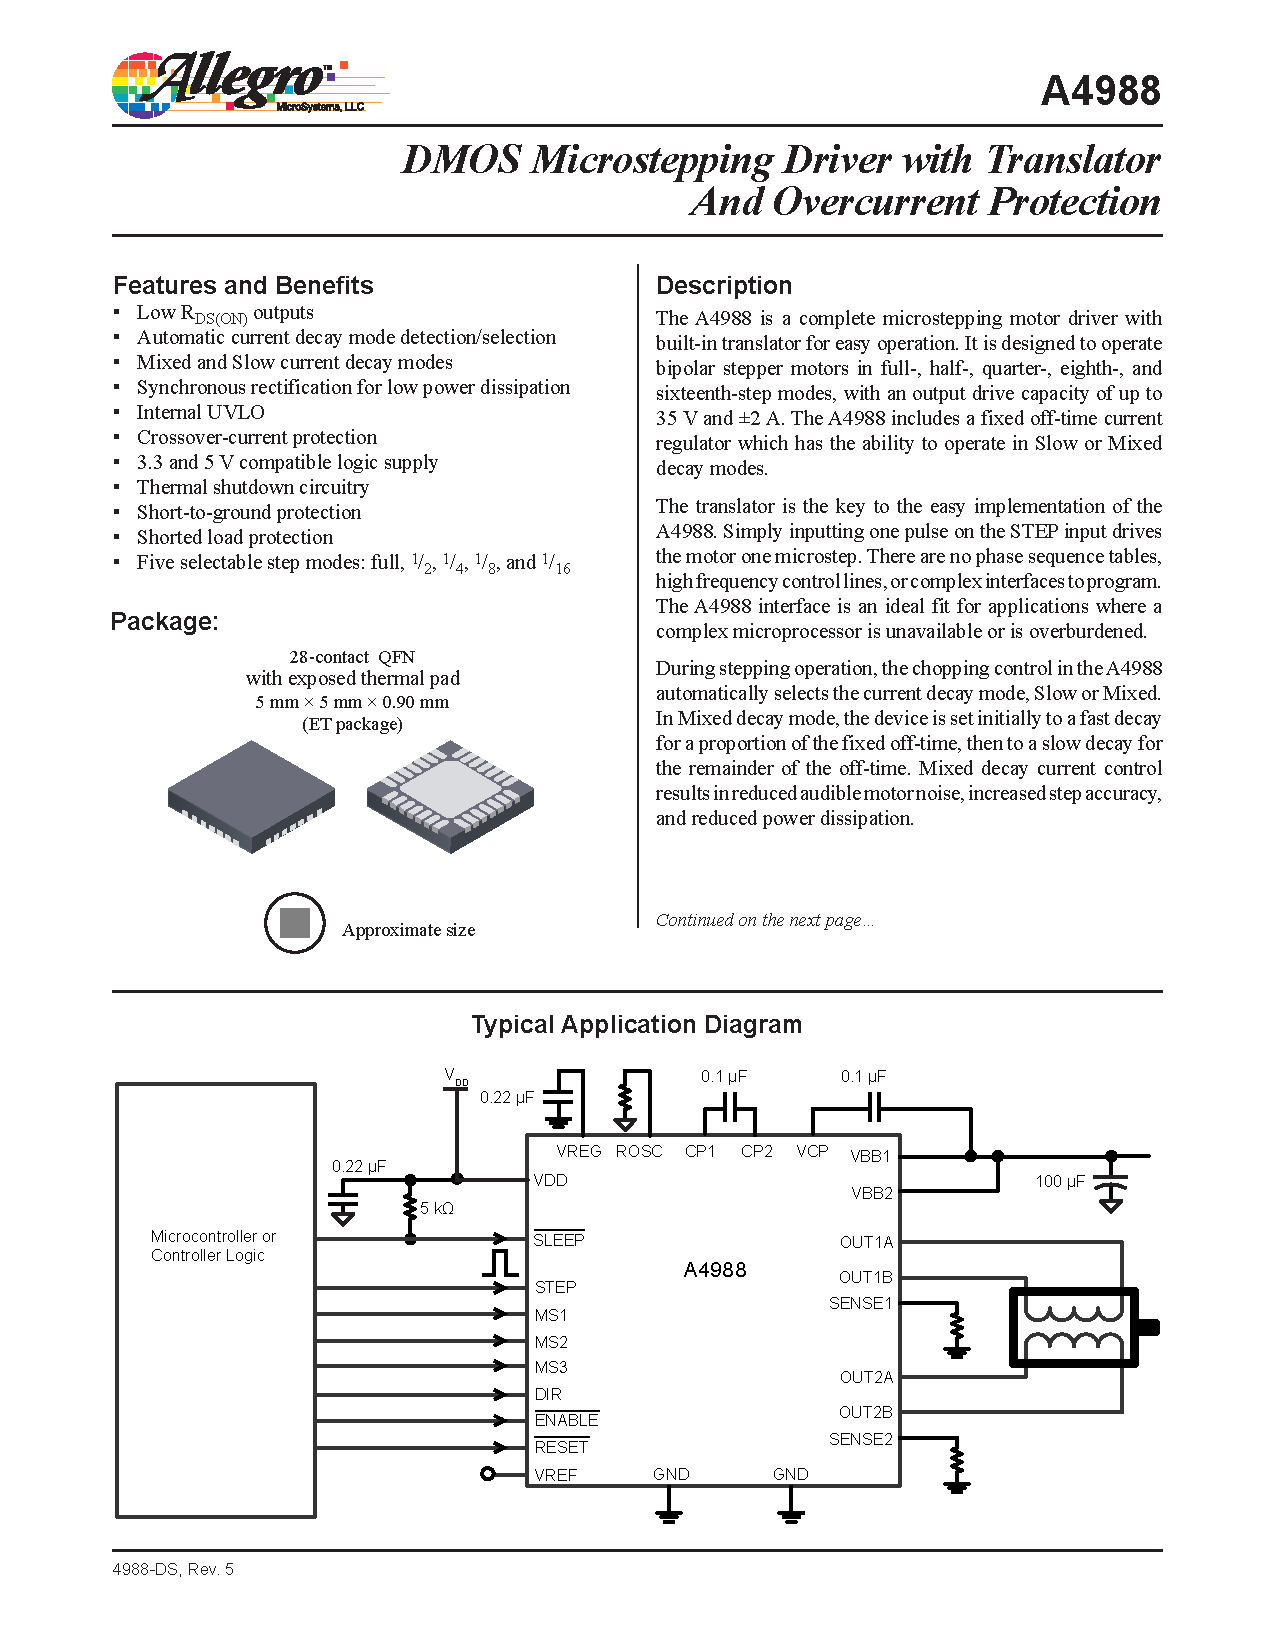
\includegraphics[width=0.7\textwidth]{A4988.jpg}
\end{figure}

\column{.5\textwidth}
\begin{figure}[ht!]
\centering
\includegraphics[width=1\textwidth]{mb_ender5.jpg}
\end{figure}

\end{columns}

\end{frame}

%%%%%%%%%%%%%%%%%%%%%%%%%%%%%%%%%%%

\end{document}